\documentclass{beamer}

\usepackage{pdfpages}
\transduration{1}
\transfade

\usetheme{Madrid} % Du kannst z. B. auch Darmstadt, Berkeley, etc. probieren

\title{Entwicklung eines Frameworks zur Robotersimulation in Jupyterlab}
\author{Philipp Mikos}
\date{\today}


% --- Fußzeile ohne Titel ---
\setbeamertemplate{footline}
{%
  \leavevmode%
  \hbox{%
    \begin{beamercolorbox}[wd=.5\paperwidth,ht=2.25ex,dp=1ex,left]{author in head/foot}%
      \usebeamerfont{author in head/foot}\hspace*{2ex}\insertshortauthor
    \end{beamercolorbox}%
    \begin{beamercolorbox}[wd=.5\paperwidth,ht=2.25ex,dp=1ex,right]{date in head/foot}%
      \usebeamerfont{date in head/foot}\insertshortdate{}\hspace*{2ex}
      \insertframenumber{} / \inserttotalframenumber\hspace*{2ex}
    \end{beamercolorbox}%
  }%
}


\begin{document}


\frame{\titlepage}



\begin{frame}{Gliederung}
  \tableofcontents
\end{frame}



\section{Einleitung}
\begin{frame}{Einleitung}
  \begin{itemize}
    \setlength{\itemsep}{1em}
    \item Entwicklung eines Frameworks zur Robotersimulation in Jupyterlab
    \item Basiert auf einer Projektarbeit 
    \item Erweiterung des Frameworks um Simulation eines Industrieroboter
    \item Hosting des Frameworks auf einem Server im IDIAL
    \item Ziel: Einsatz in der Lehre
    \item Hilfe um individuell anpassbare Übungsszenarien zu erstellen
  \end{itemize}
\end{frame}


%Im Rahmen meiner Bachelorarbeit habe ich ein Framework für die Robotersimulation entwickelt.
%Dabei wurde die Basis des Frameworks bereits in einer Projektarbeit erstellt bei der es um die Visualisierung kinematischer Kennwerte ging.
%In dieser Framework Basis konnten also bereits einfache geometrische Körper im 3-Dimensionalen Raum Transformiert werden, wobei die visuelle und interaktive Darstellung
%dieser Transformationen im Fokus stand.
%
%Die Weiterentwicklung in der Bachelorarbeit bestand dann weitestgehend darin das Framework um die Simulation eines Industrieroboters mit serieller Kinematik zu erweitern
%und auf einem Server hier im IDIAL zu hosten.
%
%Das Ziel dieses Frameworks ist es, in der Lehre eingesetzt zu werden,
%zum Beispiel in Übungen oder Vorlesungen im Bereich der Robotik, um komplexe Bewegungsabläufe und Zusammenhänge greifbarer zu machen.
%
%Der Hintergrund ist der, dass es Studierenden oft schwer fällt,
%mathematische Konzepte wie Transformationen im Raum wirklich zu verstehen.
%Konzepte wie Roll-Pitch-Yaw-WInkel oder die Denavit_hartenberg-Konvention bleiben häufig theoretisch und schwer vorstellbar.
%
%Die kinematik von Industrierobotern ist ein komplexes Thema, welches mit diesem Framework visuell aufgegriffen wird 
%
%insgesammt soll das Framework Lehrpersonen helfen, individuell anpassbare Übungsszenarien zu erstellen,
%in denen dann Studierende interaktiv und visuell mit Parametern arbeiten und experimentieren können und
%dadurch ein besseres und anwendungsnahes Verständnis für gewisse kinematische Konzepte entwickeln.

\section{Anforderungen}

\begin{frame}{Anforderungen}
  \textbf{Funktionale Anforderungen:}\vspace{0.5em}
  \begin{itemize}
    \setlength{\itemsep}{1em}
    \item Integration eines Industrieroboters mit Knickarmstruktur
    \item Umsetzung der Vorwärts- und Rückwärtstransformation
    \item Endeffektorsteuerung durch interaktive Bewegung des Koordinatensystems
    \item Bewegung im lokalen und globalen Koordinatensystem
    \item Integration einer Teach-In Funktion
    \item Manuelle Konfiguration der Gelenkwinkel
  \end{itemize}
\end{frame}



\begin{frame}{Anforderungen}
  \textbf{Nicht-Funktionale Anforderungen:}\vspace{0.5em}
  \begin{itemize}
    \setlength{\itemsep}{1em}
    \item 60 FPS und aktualisierungsrate der Animation von 60\,Hz unter typischen Systemvoraussetzungen
    \item Die GUI soll intuitiv und ohne Schulung bedienbar sein. Hauptfunktionen mit maximal drei Klicks erreichbar sein. Visuelles Feedback bei Fehlbedienung
    \item Die GUI soll so gestaltet sein, dass die Bedienung des Roboters gleichzeitig als Lernprozess dient.
  \end{itemize}
\end{frame}



\section{Entwicklungsprozess}
\begin{frame}{Entwicklungsprozess}
  \begin{itemize}
    \setlength{\itemsep}{1em}
    \item Beschaffung der 3D-Modelle von Industrierobotern
    \item Geeignete Quellen: ROS-Industrial und die Robotics Toolbox von Peter Corke
    \item 3D-Modelle performant über Framework in den Arbeitsspeicher laden mithilfe des NPZ-Formats
    \item Rendering mit pythreejs mithilfe der Klasse "Environment" $\to$ Ausgabe der 3D-Szene mit 3D-Modellen direkt im Jupyter Notebook
  \end{itemize}
\end{frame}



\begin{frame}{Entwicklungsprozess}
  \begin{itemize}
    \setlength{\itemsep}{1em}
    \item URDF-Beschreibungen laden und Parsen
    \item Informationen aus URDF-Beschreibungen wichtig um 3D-Modelle richtig zu animieren
    \item Algorithmus zu Animieren: Zeitvariable 0 $\le$ t solange um ein $\Delta$t erhöhen, wie t $\le$ 1 ist
    \item in jeder Iteration wird Rotation mehrerer Gelenke um Drehachse interpoliert
    \item Rückwärtstransformation umgesetzt auf Basis der Newton-Raphson-Methode um Roboter mit mehr als 6 Gelenken zu unterstützen
  \end{itemize}
\end{frame}


%diesmal ist das was im aufbau steht nicht interessant und das was bei entwicklungsprozess steht sollte ich am besten in stark gekürzter form hier wiedergeben

%Um die Anforderungen zu erfüllen wurde zunächst die Verfügbarkeit von 3D-Modellen für solche Industrieroboter geprüft.
%Nach längerer Recherche stellten sich ROS-Industrial und die Robotics Toolbox von Peter Corke als geeignete Quelle für die 3D-Modelle heraus.
%Der ausschlaggebene Vorteil den diese beiden Quellen gegenüber anderen Quellen hatten, war der, dass diese Quellen auch URDF-Beschreibungen zu den 3D-Modellen mitliefern,
%die im weiteren Verlauf der Entwicklung benötigt werden. Die 3D-Modelle lagen hauptsächlich im stl format vor.

%Anschließend musste eine performante Lösung gefunden werden die 3D-Modelle über das framework in den Arbeitsspeicher zu laden,
%da das Laden der stl-Dateien selbst pro Roboter auf herkömmlicher hardware im extremfall bis zu einer minute dauern konnte.
%Daher werden die stl-Dateien mithilfe eines lazy-loading algorithmus in das Binäre NPZ-Format übertragen und auf dem persistenten speicher abgelegt.
%Das laden dieser NPZ-Dateien war dann c.a 2800 mal schneller. So konnten übermäßig lange ladezeiten vermieden werden.

%Nachdem die 3D-Modelle nun performant in den Arbeitsspeicher geladen werden konnten, war es möglich diese mithilfe der wrapper-library pythreejs zu rendern.
%Dazu wird eine Klasse namens Environment verwendet, die bereits im rahmen der projektarbeit entwickelt worden ist und die Erstellung einer 3D-Szene mit Kamera, Beleuchtung
%und koordinatensystem kapselt. Diese Klasse kann der display() Funktion in einem Jupyter Notebook übergeben werden und wird somit direkt im Notebook ausgegeben.

%Abgesehen von den 3D-Modellen mussten auch noch die urdf-Bescheibungen die im .xacro format vorlagen geladen und geparsed werden.
%die URDF-Beschreibungen enthalten Informationen wie die Orientierung und Position von Gelenken und Gliedern, den Pfad zu den 3D-Modellen, welche die Glieder repräsentieren,
%Hierarchien innerhalb der kinematischen Kette sowie Minimal- und Maximal-Grenze der Gelenke und viele weitere technische Informationen.
%Diese sind wichtig um die 3D-Modelle richtig zu Animieren.

%Zum Animieren wurde bereits in der vorangegangenen Projektarbeit ein Algorithmus verwendet bei dem eine Zeitvariable 0 ≤ t solange um ein ∆t erhöht wird, wie t ≤ 1 ist.  
%Bei jedem Iterationsschritt wird dann die Transformation des zu animierenden Objekts mit t zwischen der alten und der neuen Transformation interpoliert.
%Darauf aufbauend wurde ein neuer Algorithmus entworfen, der in jeder Iteration die Rotation mehrerer Gelenke um die entsprechende Drehachse interpoliert.

%Kommen wir noch zur Rückwärtstransformation.
%Das Framework soll laut den Anforderungen die Möglichkeit bieten, die Pose des End-
%effektors sowohl über globale als auch lokale Koordinaten zu steuern. Damit
%sich die Glieder des Roboters entsprechend mitbewegen, müssen aus der Zielpose des
%Endeffektors die Gelenkkoordinaten im Konfigurationsraum bestimmt werden. Da
%auch Roboter mit mehr als 6 Gelenken, wie der LBR iiwa von KUKA, unterstützt wer-
%den sollen, wurde ein numerisches Verfahren auf Basis der Newton-Raphson-Methode
%implementiert.




\section{Aufbau}
\begin{frame}{Aufbau}
  \begin{columns}
    \begin{column}{0.6\textwidth}
      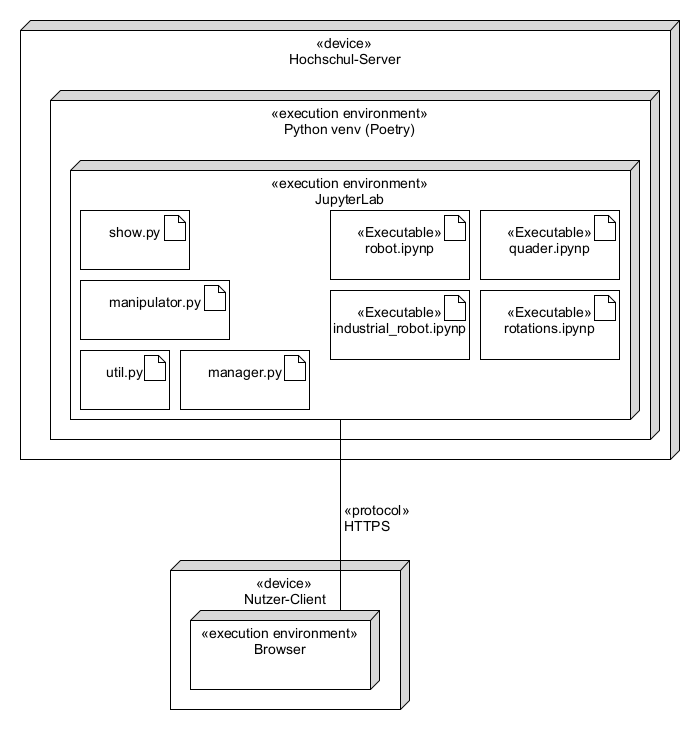
\includegraphics[width=\linewidth]{images/komDiaV2.png}
    \end{column}
    \begin{column}{0.4\textwidth}
      \textbf{Weitere Abhängigkeiten:}\vspace{0.5em}
      \begin{itemize}
        \setlength{\itemsep}{1em}
        \item Numpy
        \item SymPy
        \item SciPy
        \item pythreejs(3D Rendering)
        \item ipywidgets(GUI-Elemente)
      \end{itemize}
    \end{column}
  \end{columns}
\end{frame}








\section{Evaluation}
\begin{frame}{Evaluation}
  \begin{itemize}
    \setlength{\itemsep}{1em}
    \item Integration eines Knickarmroboters wurde umgesetzt
    \item Vorwärts- und Rückwärtstransformation ist implementiert worden 
    \item Endeffektorsteuerung durch interaktive Bewegung des Koordinatensystems wurde umgesetzt
    \item Bewegung im lokalen und globalen Koordinatensystem möglich
    \item Teach-In Funktion wurde Integriert
    \item Manuelle Konfiguration der Gelenkwinkel ist mithilfe von Schiebereglern umgesetzt worden
  \end{itemize}
\end{frame}



\begin{frame}{Evaluation}
  \begin{itemize}
    \setlength{\itemsep}{1em}
    \item Benutzerfreundliche Bedienbarkeit $\to$ müsste eine Untersuchung durch Experten oder eine Nutzerstudie erfolgen
    \item Intuitive Vermittlung kinematischer Konzepte $\to$ müsste eine Untersuchung durch Experten oder eine Nutzerstudie erfolgen
    \item performante Ausführung (60FPS und 60Hz bei aktualisierungsrate der Animation) konnte erfüllt werden
  \end{itemize}
\end{frame}





\begin{frame}{}
  \begin{center}
    \textbf{\huge Vielen Dank für Ihre Aufmerksamkeit!}  
  \end{center}
  
\end{frame}





\end{document}
